\documentclass[a4paper,12pt]{article}

\usepackage{ctex}
\usepackage[left=1.25in,right=1.25in,top=1in,bottom=1in]{geometry}
\usepackage{amsmath}
\linespread{1.5}
\usepackage{graphicx}
\usepackage{subcaption}
\usepackage{cleveref}
\usepackage{appendix} 
\usepackage{listings}
\usepackage{tcolorbox}
\usepackage{booktabs}
\usepackage{pythonhighlight}
\usepackage{array}

\title{多元线性回归分析Linnerud数据集⟩}
\author{190000000 \quad 电气类搬砖 \quad 猫九}
\date{\today}

\begin{document}
\maketitle
	
\section{多元线性回归模型}
多元线性回归分析的模型为
$$
\left\{\begin{array}{l}
	y=\beta_{0}+\beta_{1} x_{1}+\cdots+\beta_{m} x_{m}+\varepsilon \\
	\varepsilon \sim N\left(0, \sigma^{2}\right)
\end{array}\right.
$$

式中: $\beta_{0}, \beta_{1}, \cdots, \beta_{m}, \sigma^{2}$ 都是与 $x_{1}, x_{2}, \cdots, x_{m}$ 无关的末知参数, $\boldsymbol{\beta}_{0}, \boldsymbol{\beta}_{1}, \cdots, \boldsymbol{\beta}_{m}$ 称为回归系数。
现得到 $n$ 个独立观测数据 $\left[b_{i}, a_{i 1}, \cdots, a_{i m}\right]$, 其中 $b_{i}$ 为 $y$ 的观察值, $a_{i 1}, \cdots, a_{i m}$ 分别为 $x_{1}, x_{2}, \cdots, x_{m}$ 的观察值, $i=1, \cdots, n, n>m$, 由式得
$$
\left\{\begin{array}{l}
	b_{i}=\beta_{0}+\beta_{1} a_{i 1}+\cdots+\beta_{m} a_{i m}+\varepsilon_{i} \\
	\varepsilon_{i} \sim N\left(0, \sigma^{2}\right), \quad i=1, \cdots, n
\end{array}\right.
$$

记
$$
\begin{gathered}
	\boldsymbol{X}=\left[\begin{array}{cccc}
		1 & a_{11} & \cdots & a_{1 m} \\
		\vdots & \vdots & \ddots & \vdots \\
		1 & a_{n 1} & \cdots & a_{n m}
	\end{array}\right], \quad \boldsymbol{Y}=\left[\begin{array}{c}
		b_{1} \\
		\vdots \\
		b_{n}
	\end{array}\right] \\
	\boldsymbol{\varepsilon}=\left[\varepsilon_{1}, \cdots, \varepsilon_{n}\right]^{\mathrm{T}}, \boldsymbol{\beta}=\left[\boldsymbol{\beta}_{0}, \boldsymbol{\beta}_{1}, \cdots, \boldsymbol{\beta}_{m}\right]^{\mathrm{T}}
\end{gathered}
$$

表示为
$$
\left\{\begin{array}{l}
	\boldsymbol{Y}=\boldsymbol{X} \boldsymbol{\beta}+\boldsymbol{\varepsilon} \\
	\boldsymbol{\varepsilon} \sim N\left(0, \sigma^{2} \boldsymbol{E}_{n}\right)
\end{array}\right.
$$

式中: $\boldsymbol{E}_{n}$ 为 $n$ 阶单位矩阵。

\section{参数估计}
上面中的参数 $\beta_{0}, \beta_{1}, \cdots, \beta_{m}$ 用最小二乘法估计, 即应选取估计值 $\hat{\beta}_{j}$, 使当 $\beta_{j}=$ $\dot{\beta}_{j}, j=0,1, \cdots, m$ 时, 误差平方和
$$
Q=\sum_{i=1}^{n} \varepsilon_{i}^{2}=\sum_{i=1}^{n}\left(b_{i}-\hat{b}_{i}\right)^{2}=\sum_{i=1}^{n}\left(b_{i}-\beta_{0}-\beta_{1} a_{i 1}-\cdots-\beta_{m} a_{i m}\right)^{2}
$$

达到最小。为此, 令
$$
\frac{\partial Q}{\partial \beta_{j}}=0, j=0,1,2, \cdots, n
$$

得
\begin{align*}
	\frac{\partial Q}{\partial \beta_{0}}&=-2 \sum_{i=1}^{n}\left(b_{i}-\beta_{0}-\beta_{1} a_{i 1}-\cdots-\beta_{m} a_{i m}\right)=0 \\
	\frac{\partial Q}{\partial \beta_{j}}&=-2 \sum_{i=1}^{n}\left(b_{i}-\beta_{0}-\beta_{1} a_{i 1}-\cdots-\beta_{m} a_{i m}\right) a_{i j}=0, \quad j=1,2, \cdots, m_{\circ}
\end{align*}

经整理化为以下方程组:
\begin{align*}
	\beta_{0} n+\beta_{1} \sum_{i=1}^{n} a_{i 1}+\beta_{2} \sum_{i=1}^{n} a_{i 2}+&\cdots+\beta_{m} \sum_{i=1}^{n} a_{i m}=\sum_{i=1}^{n} b_{i} \\
	\beta_{0} \sum_{i=1}^{n} a_{i 1}+\beta_{1} \sum_{i=1}^{n} a_{i 1}^{2}+\beta_{2} \sum_{i=1}^{n} a_{i 1} a_{i}+&\cdots+\beta_{m} \sum_{i=1}^{n} a_{i 1} a_{i m}=\sum_{i=1}^{n} a_{i 1} b_{i} \\
	&\vdots\\
	\beta_{0} \sum_{i=1}^{n} a_{i m}+\beta_{1} \sum_{i=1}^{n} a_{i m} a_{i 1}+\beta_{2} \sum_{i=1}^{n} a_{i m} a_{i 2}+&\cdots+\beta_{m} \sum_{i=1}^{n} a_{i m}^{2}=\sum_{i=1}^{n} a_{i m} b_{i}
\end{align*}

方程组的矩阵形式为
$$
\boldsymbol{X}^{\top} \boldsymbol{X} \boldsymbol{\beta}=\boldsymbol{X}^{\top} \boldsymbol{Y}
$$

当矩阵 $\boldsymbol{X}$ 列满秩时, $\boldsymbol{X}^{\top} \boldsymbol{X}$ 为可逆方阵,解为
$$
\dot{\boldsymbol{\beta}}=\left(\boldsymbol{X}^{\mathrm{T}} \boldsymbol{X}\right)^{-1} \boldsymbol{X}^{\mathrm{T}} \boldsymbol{Y}
$$

将 $\boldsymbol{\beta}$ 代回原模型得到 $y$ 的估计值, 即
$$
\hat{y}=\hat{\beta}_{0}+\dot{\beta}_{1} x_{1}+\cdots+\dot{\beta}_{m} x_{m}
$$

而这组数据的拟合值为
$$
\hat{b}_{i}=\hat{\beta}_{0}+\hat{\beta}_{1} a_{i 1}+\cdots+\hat{\beta}_{m} a_{i m}(i=1, \cdots, n) 。
$$

记 $\hat{\boldsymbol{Y}}=\boldsymbol{X} \hat{\boldsymbol{\beta}}=\left[\hat{b}_{1}, \cdots, \hat{b}_{n}\right]^{\mathrm{T}}$, 拟合误差 $\boldsymbol{e}=\boldsymbol{Y}-\hat{\boldsymbol{Y}}$ 称为残差, 可作为随机误差 $\boldsymbol{\varepsilon}$ 的估计, 而
$$
Q=\sum_{i=1}^{n} e_{i}^{2}=\sum_{i=1}^{n}\left(b_{i}-b_{i}\right)^{2}
$$
为残差平方和。

\section{回归分析}
本例中采用Linnerud给出的关于体能训练的数据进行多元线性回归建模。数据集中被测的样本点是某健身俱乐部的20名中年男子,被测变量分为两种,第一组是身体特征指标包括体重,腰围和脉搏。第二组变量是训练结果指标,包括单杠,弯曲和跳高。

令$x_1$,$x_2$,$x_3$分别表示自变量指标\textbf{weight、waist、pulse},$y_1$,$y_2$,$y_3$分别表示因变量指标\textbf{chins 、situps 、jumps}。

求$y_1,y_2,y_3$关于$x_1$,$x_2$,$x_3$的线性回归方程,
\begin{align*}
y_1 &= c_{10} + c_{11}x_1 + c_{12}x_2 +c_{13}x_3\\
y_2 &= c_{20} + c_{21}x_1 + c_{22}x_2 +c_{23}x_3\\
y_3 &= c_{30} + c_{31}x_1 + c_{32}x_2 +c_{33}x_3
\end{align*}

计算$c$矩阵的估计值,经过计算可知:
$$
\boldsymbol{c_{ij}}=\left[\begin{array}{cccc}
	221.1277&1.5085 &-0.3932  &0.0789 \\
	41.1290 & -0.0638 & -0.0470 & -0.0470 \\
	49.4081& -0.2045 & 0.0733 & -0.0420
\end{array}\right]
$$
\begin{figure*}[!h]
	\centering
	\begin{subfigure}{0.48\textwidth}
		\centering   
		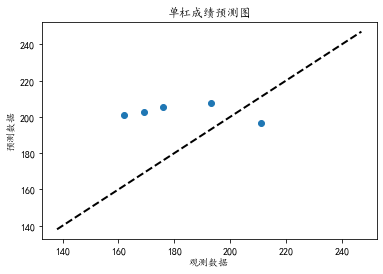
\includegraphics[scale=0.5]{pic/1.png}
		\caption{单杠成绩预测图}
		\label{fig:sub1}
	\end{subfigure}   %      \hfill  % 这个\hfill指令为插入弹性长度的空白,看情况选择加不加。
	\begin{subfigure}{0.48\textwidth}
		\centering   
		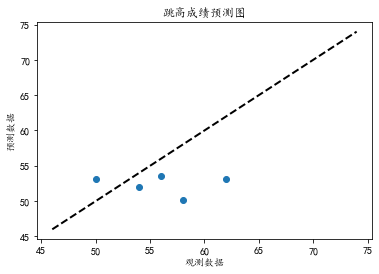
\includegraphics[scale=0.5]{pic/output_10_0.png}
		\caption{调高成绩预测图}
		\label{fig:sub2}
	\end{subfigure}
	\begin{subfigure}{0.48\textwidth}
		\centering   
		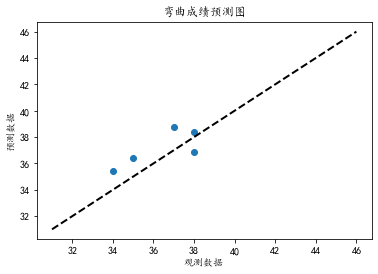
\includegraphics[scale=0.5]{pic/output_10_3.png}
		\caption{弯曲成绩预测图}
		\label{fig:sub2}
	\end{subfigure}
	\caption{
		\label{fig:total}
		因变量观测值与实际值
	}
\end{figure*}
对于多元线性回归模型的质量,可以采用均方根误差(\textbf{Root Mean Squared Error,RMSE})对模型进行评价,$RMSE$的矩阵为:
$$
\boldsymbol{R}=\left[\begin{array}{ccc}
	28.04&1.30&5.68
\end{array}\right]^{T}
$$

这里用图\ref{fig:total}观察真实值与预测值的变化关系,离中间的直线$y=x$越近的点代表预测损失越低。

由上面的回归分析图可知,对于因变量指标$y_2$(弯曲)预测值最接近真实值,误差最小,$y_2$关于$x_1$,$x_2$,$x_3$的回归方程为:
$$
y_2 = 41.1290 -0.0638x_1 -0.0470x_2 -0.0470x_3\\
$$

对于因变量指标$y_1,y_3$预测值与真实值误差较大,需要对回归系数进行假设检验和区间估计。

\newpage

\section*{附录}
\appendix

\section{代码}
\begin{python}
import pandas as pd
from sklearn.cross_decomposition import PLSRegression
from sklearn.linear_model import LinearRegression
from sklearn import datasets
from sklearn.model_selection import GridSearchCV
import numpy as np
from sklearn.model_selection import train_test_split
from sklearn import metrics
from matplotlib import pyplot as plt

dataset = datasets.load_linnerud()
col_names = dataset['feature_names'] + dataset['target_names']
data = pd.DataFrame(data= np.c_[dataset['data'], dataset['target']], columns=col_names)
x=np.array(data.loc[:,dataset['feature_names']])
y=np.array(data.loc[:,dataset['target_names'][2]])

x_train,x_test,y_train,y_test = train_test_split(x,y,random_state=1)
linreg = LinearRegression()
linreg.fit(x_train,y_train)

print(linreg.coef_,linreg.intercept_)
y_pred = linreg.predict(x_test)
print(metrics.mean_squared_error(y_test,y_pred))
print(np.sqrt(metrics.mean_squared_error(y_test,y_pred)))

plt.scatter(y_test,y_pred)
plt.plot([y.min(),y.max()],[y.min(),y.max()],'k--',lw=2)
plt.xlabel('Measured')
plt.ylabel('Predicted')
plt.show()
\end{python}

\section{Linnerud数据集}
% Table generated by Excel2LaTeX from sheet 'Sheet1'
\begin{table}[!h]
	\centering
	\caption{Linnerud数据集}
	\setlength{\tabcolsep}{6mm}
	\begin{tabular}{cccccc}
		\toprule
		\textbf{Weight} & \textbf{Waist} & \textbf{Pulse} & \textbf{Chins} & \textbf{Situps} & \textbf{Jumps} \\
		\midrule
		191   & 36    & 50    & 5     & 162   & 60 \\
		189   & 37    & 52    & 2     & 110   & 60 \\
		193   & 38    & 58    & 12    & 101   & 101 \\
		162   & 35    & 62    & 12    & 105   & 37 \\
		189   & 35    & 46    & 13    & 155   & 58 \\
		182   & 36    & 56    & 4     & 101   & 42 \\
		211   & 38    & 56    & 8     & 101   & 38 \\
		167   & 34    & 60    & 6     & 125   & 40 \\
		176   & 31    & 74    & 15    & 200   & 40 \\
		154   & 33    & 56    & 17    & 251   & 250 \\
		169   & 34    & 50    & 17    & 120   & 38 \\
		166   & 33    & 52    & 13    & 210   & 115 \\
		154   & 34    & 64    & 14    & 215   & 105 \\
		247   & 46    & 50    & 1     & 50    & 50 \\
		193   & 36    & 46    & 6     & 70    & 31 \\
		202   & 37    & 62    & 12    & 210   & 120 \\
		176   & 37    & 54    & 4     & 60    & 25 \\
		157   & 32    & 52    & 11    & 230   & 80 \\
		156   & 33    & 54    & 15    & 225   & 73 \\
		138   & 33    & 68    & 2     & 110   & 43 \\
		\bottomrule
	\end{tabular}%
	\label{tab:addlabel}%
\end{table}%
\end{document}